\subsection{ソフトウェア構築ツール}

構築ツールは、開発者がコードを書き、ビルドし、テストし、デバッグし、性能を測り、問題を発見するための支援を行う。ツールは生産性だけでなく品質にも影響する。ただし、ツールは判断を置き換えるものではない。ツールの結果をどう解釈し、どう改善につなげるかが重要である。

\subsubsection{開発環境}

開発環境、特に統合開発環境は、コード編集、コンパイル、エラー検出、ソースコード管理、ビルド、テスト、デバッグ、リファクタリング支援などを統合する。開発環境の選択は、構築効率と品質に影響する。

近年は、クラウド上の開発環境も使われる。クラウド開発環境では、ブラウザから開発でき、コンテナ化されたビルドやデプロイを利用できることがある。また、大規模言語モデルを使った AI 支援プログラミングも広がっている。AI はコード候補を生成できるが、開発者は生成されたコードをレビューし、テストし、プロジェクトへ適切に統合する責任を持つ。

\subsubsection{視覚的プログラミングとローコード/ゼロコードプラットフォーム}

視覚的プログラミングは、図形や部品を画面上で操作してプログラムを作る方法である。GUI ビルダーは、画面部品をドラッグアンドドロップで配置し、イベント処理のコード生成を支援する。

ローコード/ゼロコードプラットフォームは、視覚的な操作を中心にアプリケーションを作る環境である。ローコードは少量の手書きコードを必要とする。ゼロコードは、原則として手書きコードをほとんど必要としない。これらは、モデル駆動設計、視覚的プログラミング、コード生成の考え方に基づく。

このような環境は、開発速度を高める可能性がある。一方で、複雑な要件、性能、セキュリティ、拡張性、ベンダ依存、テスト容易性には注意が必要である。

\subsubsection{単体テストツール}

単体テストツールは、関数、クラス、モジュールなどを独立して検証するための環境を提供する。テストケースをコードとして記述し、テストランナーが自動で実行し、失敗したテストを報告する。

単体テストツールは、継続的統合と組み合わせることで価値が高まる。開発者が変更を統合するたびにテストを実行すれば、問題を早く発見できる。テストは、回帰を防ぐ安全網にもなる。

\subsubsection{プロファイリング、性能分析、スライシングツール}

プロファイリングツールは、実行中のプログラムを監視し、各文や関数がどれだけ実行されたか、どれだけ時間を使ったかを記録する。これにより、性能上のホットスポットを見つけられる。

プログラムスライシングは、ある変数や処理結果に影響し得る文の集合を計算する技法である。デバッグ、プログラム理解、最適化分析に役立つ。静的解析や動的解析を使ってスライスを求めるツールがある。

\begin{figure}[htbp]
\centering
\IfFileExists{assets/generated_figures/ch04/fig-ch04-15.png}{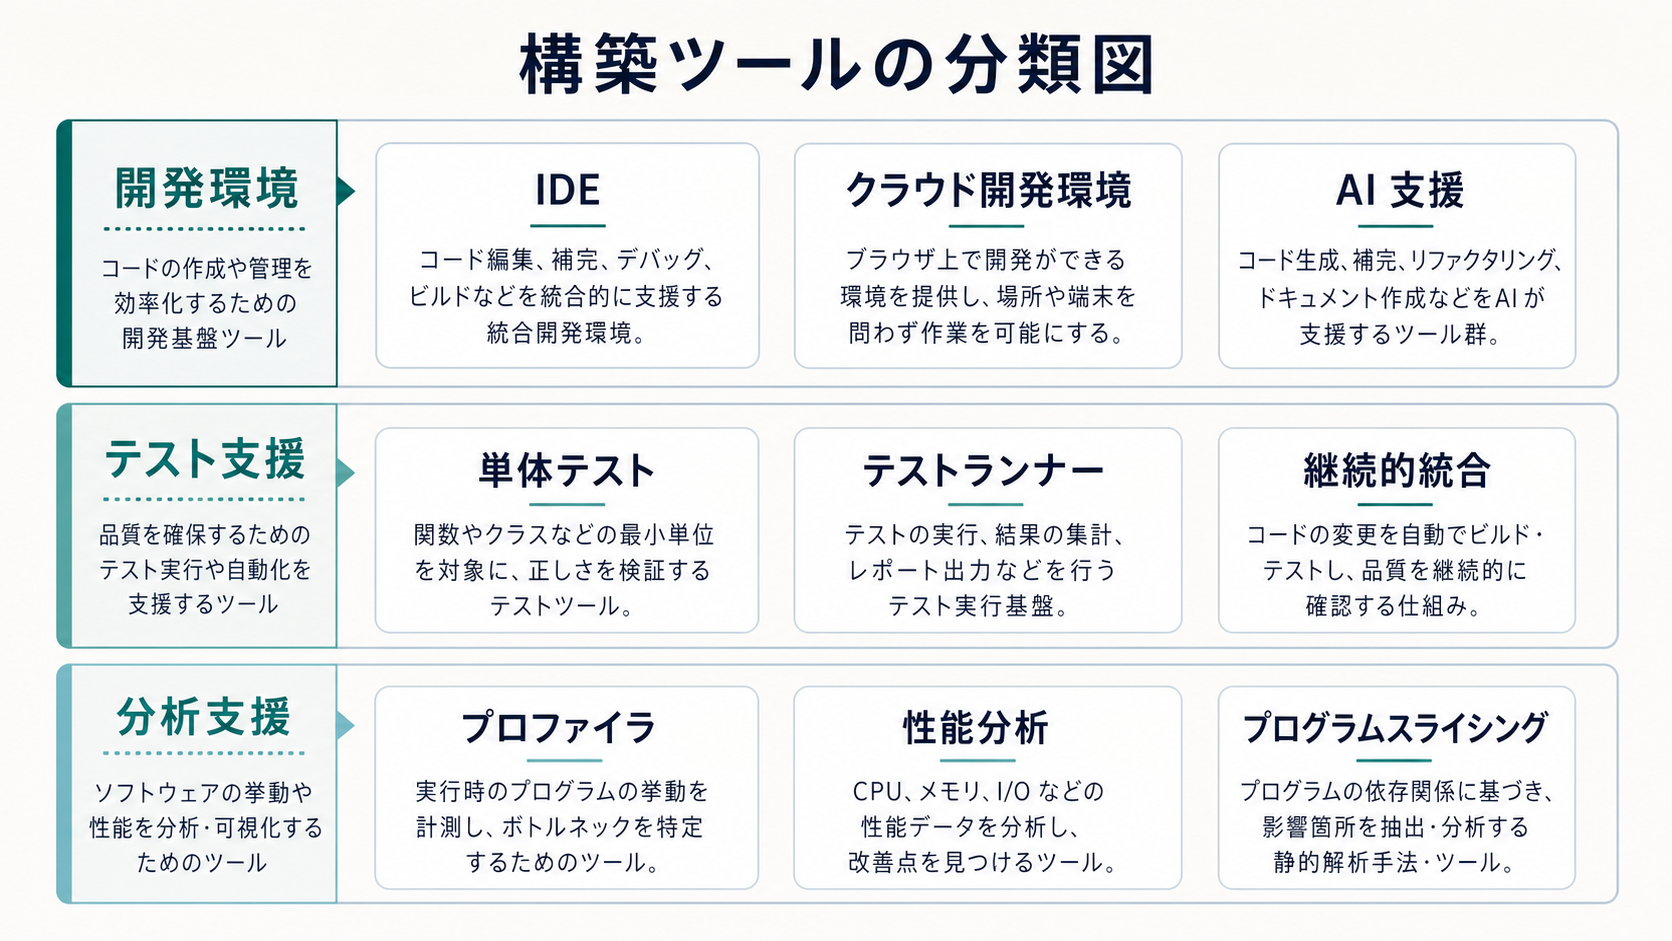
\includegraphics[width=0.96\linewidth]{assets/generated_figures/ch04/fig-ch04-15.png}}{\fbox{\parbox[c][48mm][c]{0.9\linewidth}{\centering 画像生成待ち\\構築ツールの分類図}}}
\caption{構築ツールの分類図}
\label{fig:ch04-15}
\end{figure}
